\subsection{El juego}\label{juego}
El juego definida por la RAE es una actividad  recreativa o de competición sometida a reglas por el entretenimiento. Sin embargo más que ello es parte fundamental parael desarrollo y aprendizaje de cualquier individuao. Esta actividad contribuye a la maduración, potencia cognitiva, desarrollo emocional, vehículo emocional que contribuye para aprender nuevas habilidades y conceptos a través de su propia experiencia.

El juego refleja la percepción de sí mismos, de otras personas y del mundo que nos rodea. Por ello mismo cuenta con 5 grandes ventajas:
\begin{itemize}
	\item El juego otorga placer y felicidad.
	\item En el juego no se tiene miedo al error.
	\item Fomenta la creatividad.
	\item Práctica de creación de estrategias y colaboración.
	\item El juego es el aprendizaje natural de las personas.
\end{itemize}
	
\subsubsection{Teorías del aprendizaje}
Es el estudio del aprendizaje que concierne al proceso por el que ocurre según el libro "Teorías del aprendizaje" \cite{libroTeoApr}. Pues se necesita comprender algunas suposiciones generales de las teorías que sustentan el aprendizaje humano y de la forma en la que se construyen sus principios.

Las teorías más reconocidas sobre el aprendizaje son:
\begin{itemize}
	\item Gestalt: reestructuración perceptual.
	\item Piaget: Constructivismo genético.
	\item Vygotsky: Teoría sociocultural.
	\item Ausbel: Teoría del aprendizaje significativo.
	\item Bruner: Teoría cognitiva.
\end{itemize}

Aquella más cercana al juego para el trabajo a realizar es la teoría de Bruner. Pues el jugador que contempla es epistémico social, inserto en una cultura y estructurado por un lenguaje. La inteligencia esta relacionada con 3 etapas de desarrollo para conocer: ejecución, impresión o imagen y significado simbólico. La evaluación está enfocada al estudio integral de los procesos cognoscitivos y los cambios que se originan.


\subsubsection{Los videojuegos como medio de comunicación}
Los videojuegos gracias a sus características de alcance masivo y presentación interactiva al usuario, son considerados parte de las TIC (tecnologias de la información y comunicación). Estos son más atractivos e influyentes dado que se enfoca a el ocio y entretenimiento de las personas. 
Es así como podemos ver incluso a los videojuegos usados como publicidad, puede ser de manera implícita donde se muestre marcas o productos dentro de un escenario o situación del juego o explícita donde el mismo juego presenta a la marca mostrando sus cualidades y ventajas (en la mayoría de los casos de forma exagerada). Además podemos ahora combinar la expansión que nos da el internet junto con la diversión de un videojuego, posibilitando a los jugadores la capacidad de promover los productos que han probado y enseñarlo a los demás jugadores.


\subsubsection{Serious games}
Aquí podemos aprovechar la creación de un serious game, pues son los juegos digitales con una finalidad explícita para el aprendizaje más allá del entretenimiento sin ser pensados en la diversión. Tienen su interés en el desarrollo de las competencias, mediante actividades interactivas basadas en el juego.
Contribuyen al desarrollo de la coordinación ojo-mano, agudeza visual, reacción, atención múltiple, aptitud relacional, motivación, tolerancia a la frustración, toma de riesgos, resolución de problemas y toma de desiciones, así como la reflexión estratégica, la creatividad, cooperación y sentido de innovación {marqués, 2010, p.276}. Así mismo el jugador mejora el desempeño y se adentra a la experimentación, dada una situación simulada en la realidad virtual sin tener que enfrentar los riesgos de la realidad. 

La gamificación y game-based learning son herramientas que persiguen el mismo objetivo de atraer y hacer practicar experiencias para memorizar y retener contenidos. Pueden usarse como ayuda para crear un serious game.

La gamificación es el uso de elementos de juego y técnicas de diseño para potenciar la motivación y compromiso de los jugadores. Mientras game-based learning se refiere al área cognitiva y apariencia donde debe crearse una experiencia de aprendizaje positiva.

En el siguiente cuadro\cite{gabale} establecemos las diferencias más destacadas en ambás técnicas.

\begin{table}[htbp]
	\centering
	\caption{Diferencias entre gamificación y game-based learning}
	\label{gabale}
	\begin{tabular}{ll}
		Gamificación                                                        & Game-based learning                                                         \\
		Incluir los mecanismos de los juegos a situaciones de aprendizaje   & Usar los juegos para crear una experiencia de aprendizaje                   \\
		Existen como motivadores puntos de experiencia, logros e incentivos & La experiencia va dirigida al pensamiento crítico y resolución de problemas \\
		Enriquece la ambientación y simulación del aprendizaje              & Ambientación y simulación controlada a solo eventos positivos              
	\end{tabular}
\end{table}

\subsubsection{Motivos para jugar}
El área de interés para el desarrollo del trabajo es la gamificación, para ello la parte importante a conocer son los diferentes motivantes que tiene una persona al jugar.

Para determinar el perfil motivacional se tomará la "rueda de motivos"\ref{fig:rm} definida por Valderrama\cite{valde}, donde se define motivos de aproximación; aquellas personas sociales y buscan la convivencia y motivos de evitación; aquellas personas que prefieren la seguridad y estancia individual.
\begin{figure}
	\centering
	\caption{Rueda de motivos de Beatris Valderrama}
	\label{fig:rm}
	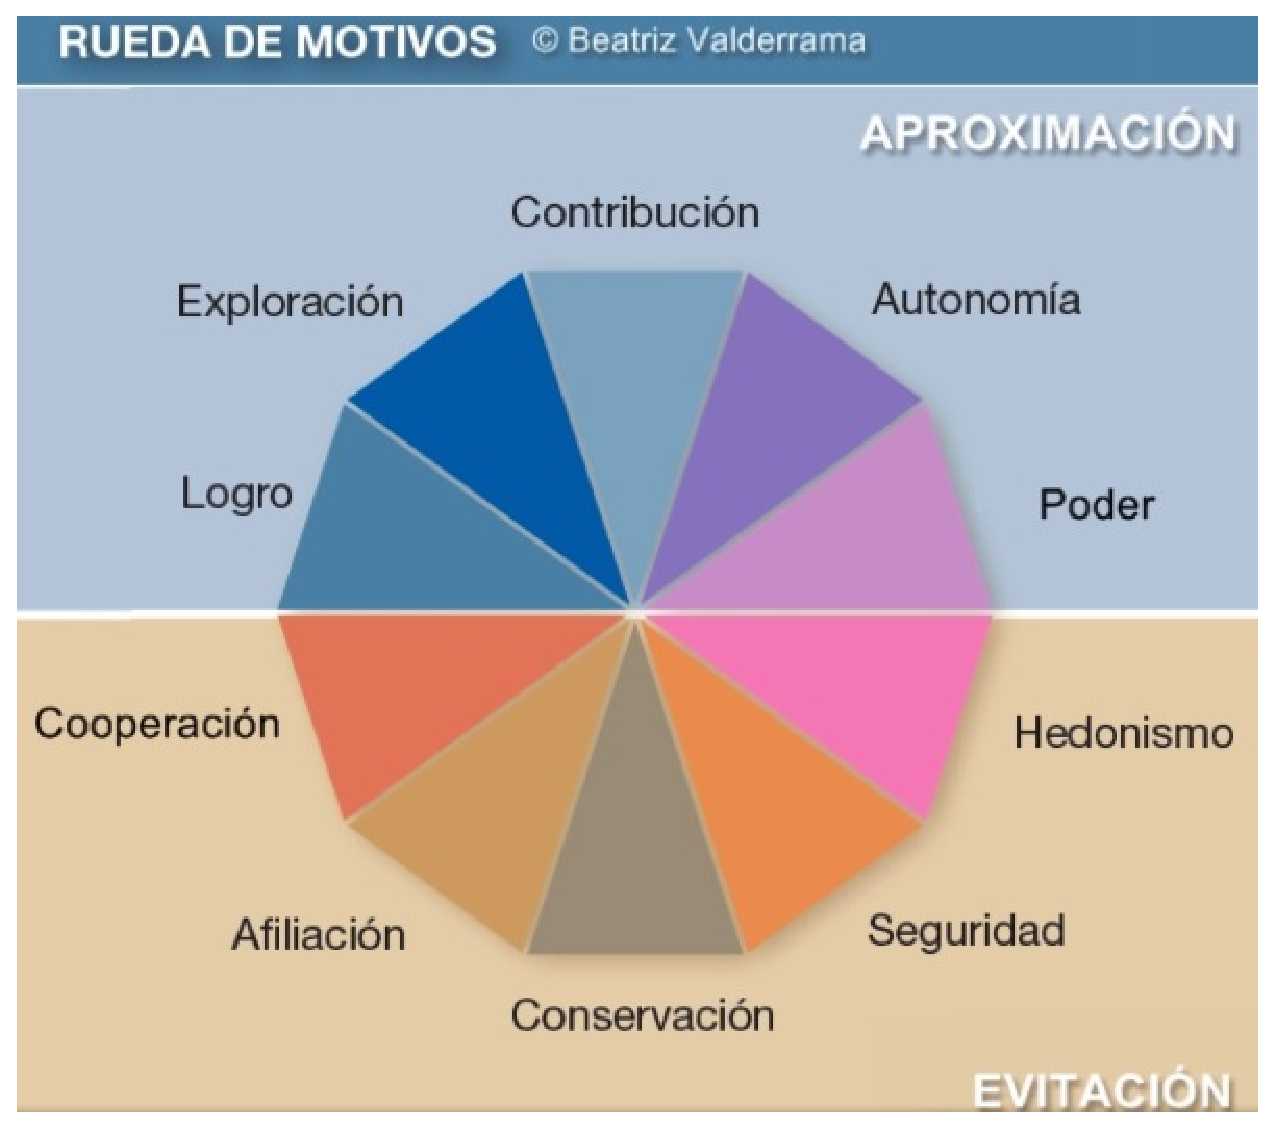
\includegraphics[width=0.5\textwidth]{imagenes\rueda-de-motivos}
\end{figure}

Es así como tenemos en contra partes diferentes motivos dependiendo del jugador obejtivo, que son la búsqueda de:
\begin{itemize}
	\item Logros o hedonismo
	\item Exploración o seguridad
	\item Contribución o conservación
	\item Autonomía o afiliación
	\item Poder o cooperación
\end{itemize}
 